\section{Data and MC samples, event selection criteria, basic plots}
\label{sec:samples}

%%%%%%%%%%%%%%%%%%%%%%%%%%%%%%%%%%%%%%%%
\subsection{Data samples}
\label{sec:datasamples}

The analysis uses the data samples collected by CMS during the 2017 and 2018 running periods.
The events were collected with
% the {\tt HLT\_Dimuon25\_Jpsi} dimuon trigger
two dimuon triggers, for the \jpsi and the \psip cases,
the HLT paths being called {\tt HLT\_Dimuon25\_Jpsi} and {\tt HLT\_Dimuon18\_PsiPrime}, 
respectively.
%
The trigger requires an opposite-sign muon pair invariant mass, 
in the ranges 2.9--3.33\GeV for the \jpsi and 3.35--4.05\GeV for the \psip,
%in the range 2.9--3.33\GeV,
with a distance of closest approach between the two muons smaller than 0.5\cm and
a fit of the positions and momenta of the two muon candidates to a common vertex
(``dimuon vertex fit") $\chi^2$ probability larger than 0.5\%.
In addition, the dimuon transverse momentum must be 
larger than 24.9\GeV, for the \jpsi, or 17.9\GeV, for the \psip.
No explicit \pt\ requirement was imposed on the single muons at trigger level.
The dimuon rapidity is restricted to $\abs{y} < 1.25$ because this is the most 
interesting kinematical region for the physics analyses and also where the 
measurements have the best resolutions.
Including forward rapidity dimuons 
(the full CMS rapidity coverage in Run~2 is $\abs{y} < 2.5$)
would have implied increasing the \pt threshold to larger values,
to keep the total trigger rate within the allocated trigger bandwidth.

The integrated luminosity adds up to 103.3\fbinv, 
distributed as 42.0 and 61.3\fbinv for 2017 and 2018, respectively.
These values are computed with the standard \texttt{brilcalc} tool~\cite{bib:brilcalc}
and take into consideration that we only use data collected in the certified lumisections,
as listed in the following JSON files, one per year of data taking:
\begin{itemize}
\item \texttt{Cert\_294927-306462\_13TeV\_UL2017\_Collisions17\_MuonJSON}
\item \texttt{Cert\_314472-325175\_13TeV\_Legacy2018\_Collisions18\_JSON\_MuonPhys}
\end{itemize}
It should be kept in mind that the polarization measurement is completely 
independent of the exact value of the integrated luminosity, which is only
reported to offer a qualitative measure of the size of the analysed event sample.

The ntuples were produced with the so-called ``UltraLegacy production", 
the latest available reconstruction software.
Table~\ref{tab:PDs} lists all the (MiniAOD) samples and respective run ranges.

\begin{table}[h]
\centering 
\caption{Data samples and run ranges used in the current analysis.}
\label{tab:PDs}
\begin{tabular}{lr}\hline
Data sample               & Run range \\ \hline
Run2017B-09Aug2019\_UL2017-v1 & 297047--299329 \\
Run2017C-09Aug2019\_UL2017-v1 & 299368--302029 \\
Run2017D-09Aug2019\_UL2017-v1 & 302031--302491 \\
Run2017E-09Aug2019\_UL2017-v1 & 303824--304671 \\
Run2017F-09Aug2019\_UL2017-v1 & 305040--305364 \\ \hline
Run2018A-12Nov2019\_UL2018\_rsb-v1 & 315257--316995 \\
Run2018B-12Nov2019\_UL2018-v1 & 317080--319310 \\
Run2018C-12Nov2019\_UL2018-v1 & 319337--320008 \\
Run2018D-12Nov2019\_UL2018-v1 & 320500--321068 \\ \hline
\end{tabular}
\end{table}

The reconstructed data were processed ensuring that both reconstructed muons 
must match, in pseudorapidity and azimuthal angle, those that triggered the detector readout.
Both muon tracks must have more than five hits in the tracker, 
at least one of them being in a pixel detector layer.
They must also fulfill the other standard quarkonium muon selection cuts 
(the so-called ``soft-muon selection"~\cite{bib:softmuon2}).

%%%%%%%%%%%%%%%%%%%%%%%%%%%%%%%%%%%%%%%%
\subsection{Monte-Carlo samples}
\label{sec:mcsamples}

The analysis also uses simulated (MC) event samples, 
generated with the \PYTHIA\,8 event generator~\cite{bib:Pythia},
with the standard charmonium production settings.
The MC samples are exclusively composed of prompt mesons (pure signal).
The generated \jpsi and \psip 
mesons only decay to dimuons, to avoid wasting CPU.
The decays are isotropic, i.e.\ reflecting unpolarized production.
Final state QED radiation is generated
for the muons through the 
\PHOTOS\,3.61 package~\cite{PHOTOS2}.
The simulated events include multiple $\Pp\Pp$ interactions in the same
or nearby beam crossings (pileup), with a distribution matching the one observed in data
(the average number of pileup interactions was 32 in the 2017--2018 period). 
The simulated events are then processed through a detailed simulation of the CMS detector,
based on the \GEANTfour package~\cite{bib:geant4}, 
using the same trigger and reconstruction algorithms as used to collect and process the data. 
These samples are independently generated for each of the two years and are
expected to faithfully reproduce the running conditions of the CMS experiment 
during the data collection periods.
All samples are generated with the single muons in the kinematical window 
$\pt > 4$\GeV and $|\eta| < 1.5$.

Some of the MC samples were ``officially produced".
%(and are in DAS, \texttt{cmsweb.cern.ch/das/}).
%the initial samples have the name JpsiToMuMu\_JpsiPt8\_TuneCP5\_13TeV-pythia8
%followed by:
%\begin{itemize}
%\item \texttt{RunIISummer19UL17MiniAOD-PUForMUOVal\_106X\_mc2017\_realistic\_v6-v2},
%\item \texttt{RunIISummer19UL18MiniAOD-106X\_upgrade2018\_realistic\_v11\_L1v1-v2}.
%\end{itemize}
They were complemented by additional MC samples, generated ``privately"
following the procedures used in the official production, 
so that the final results are not significantly affected by the statistical uncertainties 
of the simulated samples.
%
%
%with the name Charmonium\_JpsiToMuMu\_Pt25\_46\_TuneCP5\_13TeV-pythia8
%followed by:
%\begin{itemize}
%\item \texttt{RunIISummer20UL17MiniAOD-106X\_mc2017\_realistic\_v6-v1},
%\item \texttt{RunIISummer20UL18MiniAODv2-106X\_upgrade2018\_realistic\_v16\_L1v1-v1}.
%\end{itemize}
%For the \psip case, all the MC files were generated ``privately", 
%following the procedures used in the official production.

To improve the statistical uncertainties at high \pt, several complementary 
\jpsi MC samples were generated. They are used in four exclusive ranges:
25--45; 45--50; 50--70; 70--120\GeV. 
For the \psip case, a single high-statistics MC sample was produced.

%\vfill\newpage

%%%%%%%%%%%%%%%%%%%%%%%%%%%%%%%%%%%%%%%%
\subsection{Event selection criteria and definition of analysis samples}
\label{sec:eventsel}

For easy reference, we list in this section the offline event selection criteria used to define the
``final-analysis event sample":
\begin{itemize}
\item Single muon kinematical cuts: $\pt > 5.6$\GeV and $|\eta| < 1.4$;
\item Dimuon rapidity cuts: $|y| < 1.2$;
\item Dimuon \pt cuts: $25 < \pt < 120$\GeV (\jpsi) or $20 < \pt < 100$\GeV (\psip);
\item Dimuon mass: $2.92 < m < 3.28$\GeV (\jpsi) or $3.4 < m < 4.0$\GeV (\psip);
\item Dimuon vertex fit $\chi^2$ probability larger than 1\%.
\end{itemize}

The observables used in all of these event selection steps are computed 
with the standard Onia2MuMu package, 
which has been used in analogous ways in all the CMS quarkonium analyses 
made on the basis of the Run~1 data, 
as well as in the paper reporting quarkonium production cross sections with the 2015 data (BPH-15-005).
The source code, continuously updated within the BPH PAG throughout the last 10 years,
can be consulted in Ref.~\cite{bib:onia2mumu}.

\begin{figure}[h]
\centering
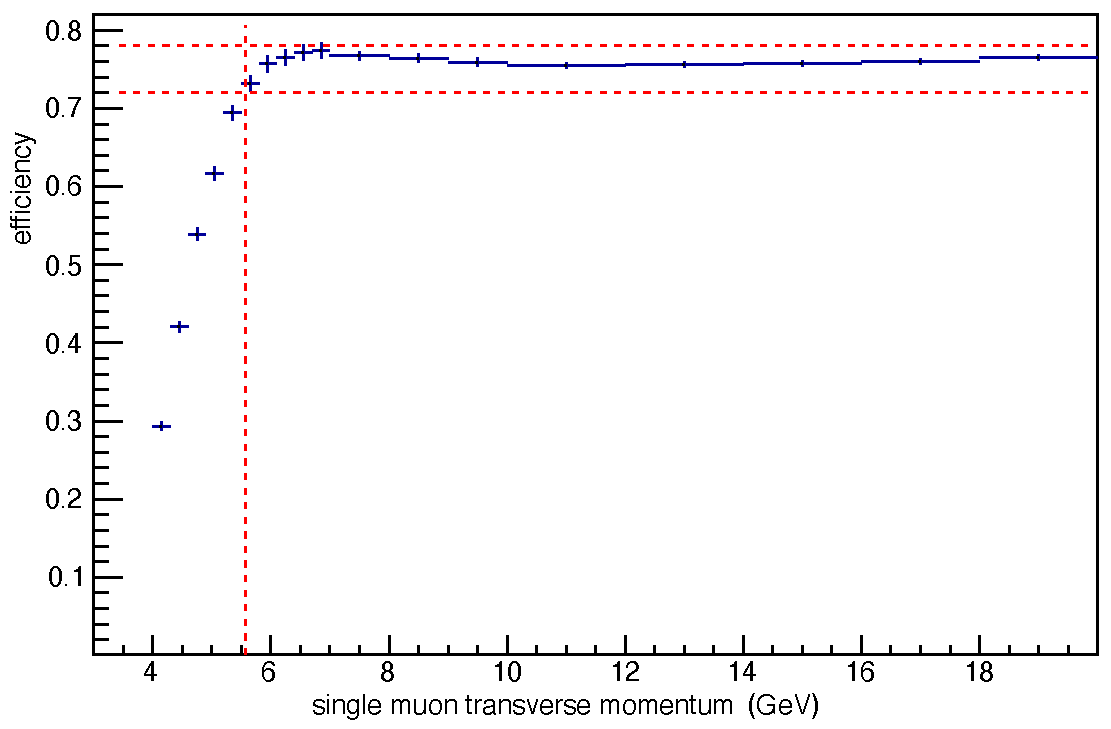
\includegraphics[width=0.75\textwidth]{Figures/chapter2/efficiency_vs_ptmuon.pdf}
\caption{Single muon efficiency as a function of \pt, as evaluated from the simulated events.}
\label{fig:muon_eff}
\end{figure}

The single muon \pt cut is set at 5.6\GeV so that all the selected muons have detection efficiencies
that vary by less than 5\%. as can be seen in Fig.~\ref{fig:muon_eff}.
In other words, all the analysed events have both muons in the ``plateau" region of the
detection efficiency.
It is important to keep in mind that the polarization measurement is insensitive to 
the absolute magnitude of the detection efficiencies, so that we only need to worry about the 
variations of efficiency within the analysed sample matter.
By avoiding the \pt dependent ``turn-on" region of the efficiency curve,
we minimise the potential residual effects of a less-than-perfect efficiency correction,
so that the results become almost unaffected by the uncertainties on the assumed efficiencies.

%\vfill\newpage

The \jpsi polarization parameter \lth is measured, in the helicity frame and as a function of \pt, 
using the \abscosth distributions measured in six independent event samples, 
defined by two ranges in the dimuon lifetime (prompt and non-prompt) 
and three in the dimuon mass (\jpsi region, left and right sidebands):

\begin{itemize}

\item PR: $|c\tau| < 50~\mu$m; NP: $100 < c\tau < 500~\mu$m;

\item \jpsi mass region: 3.0--3.2~GeV; LSB: 2.92--2.95~GeV; RSB: 3.21--3.28~GeV.

\end{itemize}

The \psip analysis is done in a completely analogous way, simply replacing the 
\jpsi mass regions by the corresponding \psip regions:

\begin{itemize}

\item PR: $|c\tau| < 50~\mu$m; NP: $100 < c\tau < 500~\mu$m;

\item \psip mass region: 3.57--3.81~GeV; LSB: 3.4--3.52~GeV; RSB: 3.82--4.0~GeV.

\end{itemize}

The NP and 3.0--3.2~GeV 2D region includes the non-prompt \jpsi mesons (from B decays) 
plus a background contribution from non-prompt ``mass continuum" muon pairs.
The PR and 3.0--3.2~GeV 2D region (which we label as ``Peak") 
contains the prompt \jpsi mesons plus background contributions from prompt 
``mass continuum" muon pairs and ``non-prompt" \jpsi mesons.

The MC samples are exclusively composed of prompt \jpsi mesons.

\begin{figure}[ht]
\centering
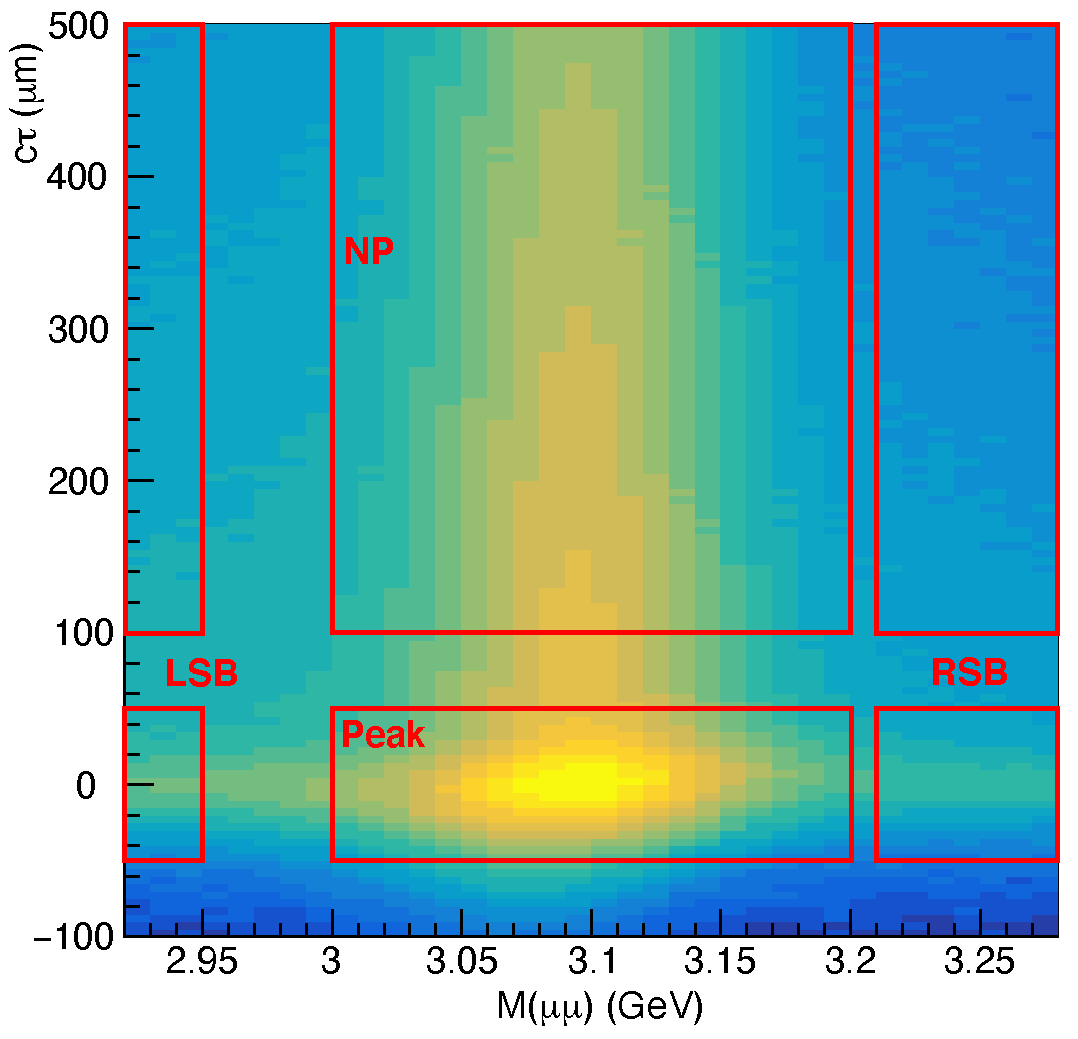
\includegraphics[width=0.45\linewidth]{Figures/chapter2/2D_map_ctau_vs_mass_jpsi_2018.pdf}
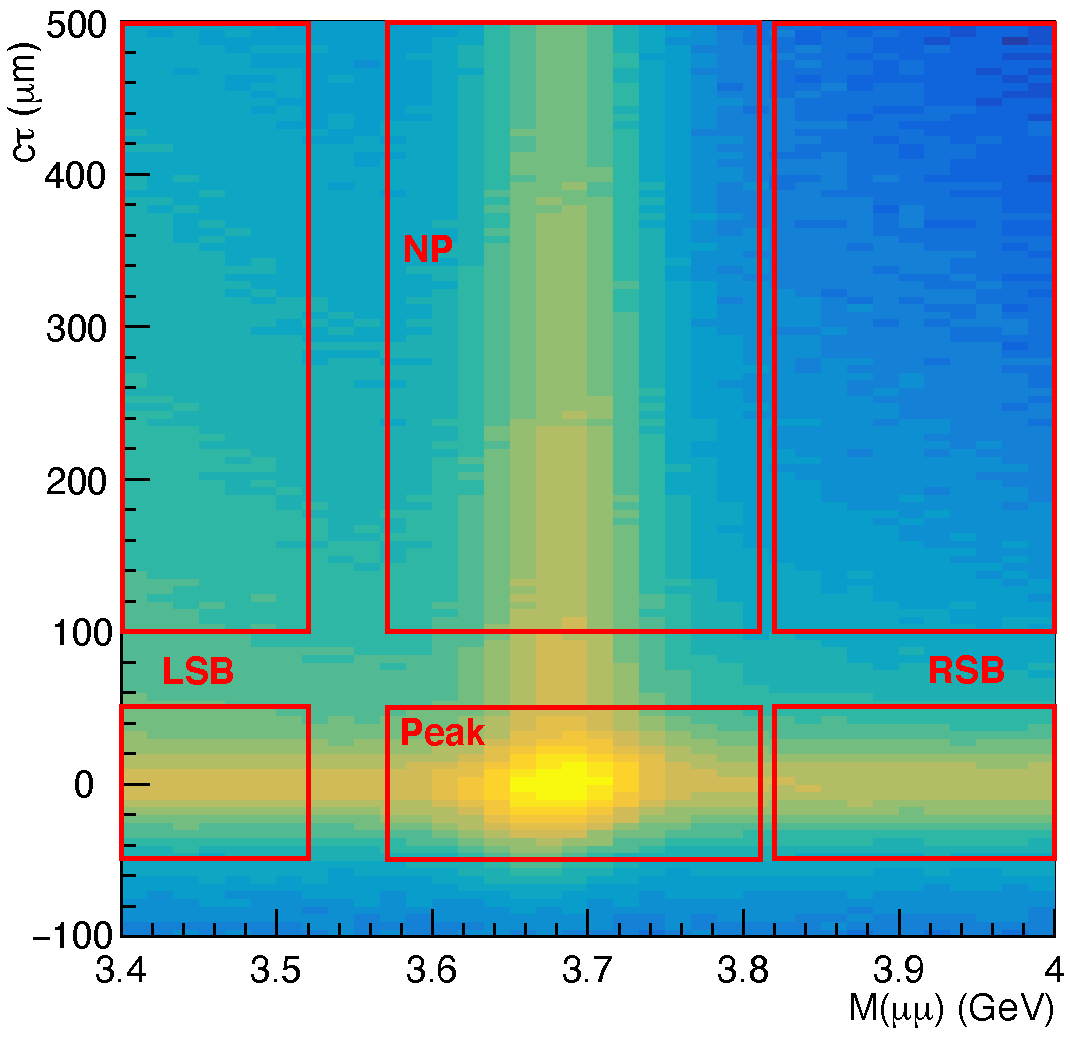
\includegraphics[width=0.45\linewidth]{Figures/chapter2/2D_map_ctau_vs_mass_psip_2018.pdf}
\caption{Two-dimensional event distribution in the dimuon lifetime vs.\ mass dimensions,
for the 2018 \jpsi (left) and \psip (right) data samples,
showing the rectangular windows defining the six regions used in the analysis.
The Peak windows include the prompt signal as well as the two background contaminations.
The five ``control windows" are used to evaluate the \abscosth distributions of those backgrounds.}
\label{fig:2D_ctau_vs_mass_map}
\end{figure}

For illustration purposes, the six windows used in the \jpsi and \psip analysis 
are graphically represented in Fig.~\ref{fig:2D_ctau_vs_mass_map}.
The dimuon mass resolution at the \jpsi mass is around 20--40\MeV, 
depending on dimuon rapidity and \pt, 
so that the range $3.0 < m < 3.2$\GeV corresponds to a coverage of around $\pm \,3~\sigma$.
The dimuon pseudo-proper lifetime observable, $c\tau$, is the distance between the dimuon vertex 
and the primary vertex. It is measured with a resolution of around 20--30~$\mu$m, 
so that the range $|c\tau| < 50\,\mu$m corresponds to a coverage of around 2~$\sigma$.
The primary vertex is selected among all the reconstructed proton-proton collision vertices in the event 
as the one closest to the line extrapolating the dimuon momentum back to the beam line.

The \jpsi polarization is measured in 19 \pt bins, of widths increasing with increasing \pt:
\begin{itemize}
\item 10 bins of 2.5 GeV in the range 25--50 GeV;
\item 6 bins of 5 GeV in the range 50--80 GeV;
\item 2 bins of 10 GeV in the range 80--100 GeV;
\item 1 bin of 20 GeV in the range 100--120 GeV.
\end{itemize}

Given the smaller event sample, 
the \psip polarization measurement is made in only 8 \pt bins, of variable width:
\begin{itemize}
\item 4 bins of 5 GeV in the range 20--40 GeV;
\item 3 bins of 10 GeV in the range 40--70 GeV;
\item 1 bin of 30 GeV in the range 70--100 GeV.
\end{itemize}

In each of those \pt bins, the \abscosth distribution (or ratio of distributions) 
is analysed in 20 equidistant bins between 0 and 1.

\vfill\newpage

%%%%%%%%%%%%%%%%%%%%%%%%%%%%%%%%%%%%%%%%
\subsection{Event yields per year of data taking}
\label{sec:yields}

After applying the event selection criteria described in the previous section, 
we are left with almost 15 million prompt and almost 11 million non-prompt 
\jpsi dimuons with \pt between 25 and 120\GeV. 
The number of \psip events is significantly smaller: 
2.1 million prompt and 1.3 million non-prompt.
All the event yields are collected in Tables~\ref{tab:yields-jpsi} and~\ref{tab:yields-psi2S}.

\begin{table}[h!]
\centering 
\caption{Event yields of the measured and simulated \jpsi samples,
for the 2017 and 2018 sets, per \pt range (in GeV).}
\label{tab:yields-jpsi}
%\footnotesize
\small
\begin{tabular}{cl|cccc|c}
\hline
\multicolumn{2}{c}{2017} & $[25, 45]$ & $[45, 50]$ & $[50, 70]$ & $[70, 120]$ & $[25, 120]$ \\
\hline
\multirow{6}{*}{\rotatebox[origin=c]{90}{Data}} 
& Prompt signal region (Peak) & 5.380 M & 0.209 M & 0.282 M & 0.073 M & 5.944 M \\
& Non-prompt region (NP) & 3.883 M & 0.180 M & 0.253 M & 0.068 M & 4.384 M \\
& Prompt left mass SB (PRLSB) & 44.6 k & 2.1 k & 3.0 k & 1.0 k & 50.7 k \\
& Prompt right mass SB (PRRSB) & 52.9 k & 2.9 k & 4.5 k & 1.6 k & 61.9 k \\
& Non-prompt left mass SB (NPLSB) & 62.1 k & 2.9 k & 4.0 k & 1.0 k & 70.1 k \\
& Non-prompt right mass SB (NPRSB) & 66.9 k & 3.2 k & 4.5 k & 1.2 k & 75.9 k \\
\hline
MC & only Peak region & 20.508 M & 1.555 M & 1.999 M & 1.275 M & 25.337 M \\
\hline
\hline
\multicolumn{2}{c}{2018} & $[25, 45]$ & $[45, 50]$ & $[50, 70]$ & $[70, 120]$ & $[25, 120]$ \\
\hline
\multirow{6}{*}{\rotatebox[origin=c]{90}{Data}} 
& Prompt signal region (Peak) & 7.982 M & 0.307 M & 0.416 M & 0.107 M & 8.813 M \\
& Non-prompt region (NP) & 5.746 M & 0.265 M & 0.373 M & 0.100 M & 6.484 M \\
& Prompt left mass SB (PRLSB) & 69.2 k & 3.2 k & 4.7 k & 1.4 k & 78.5 k \\
& Prompt right mass SB (PRRSB) & 79.5 k & 4.4 k & 6.8 k & 2.4 k & 93.1 k \\
& Non-prompt left mass SB (NPLSB) & 97.1 k & 4.4 k & 6.2 k & 1.7 k & 109.4 k \\
& Non-prompt right mass SB (NPRSB) & 101.2 k & 4.8 k & 6.5 k & 1.8 k & 114.2 k \\
\hline
MC & only Peak region & 20.984 M & 1.590 M & 1.760 M & 1.599 M & 25.933 M \\
\hline
\end{tabular}
\end{table}

\begin{table}[ht]
\centering 
\caption{Event yields of the measured and simulated \psip samples,
for the 2017 and 2018 sets, in the full \pt range.}
\label{tab:yields-psi2S}
\small
\begin{tabular}{cl|c}
\hline
\multicolumn{2}{c}{2017} & $[20, 100]$ \\
\hline
\multirow{6}{*}{\rotatebox[origin=c]{90}{Data}} 
& Prompt signal region (Peak) & 0.854 M \\
& Non-prompt region (NP) & 0.543 M \\
& Prompt left mass SB (PRLSB) & 162.0 k \\
& Prompt right mass SB (PRRSB) & 183.9 k\\
& on-prompt left mass SB (NPLSB) & 147.1 k\\
& Non-prompt right mass SB (NPRSB) & 56.7 k \\
\hline
MC & only Peak region & 5.572 M  \\
\hline
\hline
\multicolumn{2}{c}{2018} & $[20, 100]$ \\
\hline
\multirow{6}{*}{\rotatebox[origin=c]{90}{Data}} 
& Prompt signal region (Peak) & 1.276 M \\
& Non-prompt region (NP) & 0.808 M \\
& Prompt left mass SB (PRLSB) & 242.9 k \\
& Prompt right mass SB (PRRSB) & 275.6 k\\
& on-prompt left mass SB (NPLSB) & 220.6 k\\
& Non-prompt right mass SB (NPRSB) & 84.9 k \\
\hline
MC & only Peak region & 6.660 M  \\
\hline
\end{tabular}
\end{table}

\vfill\newpage

%%%%%%%%%%%%%%%%%%%%%%%%%%%%%%%%%%%%%%%%
\subsection{Illustrations of some kinematical distributions}
\label{sec:basicplots}

The next figures illustrate the dimuon mass, \pt, rapidity, and lifetime distributions, 
and how the measured and simulated spectra compare to each other.
These illustrations are made with the 2018 \jpsi data.

\begin{figure}[h]
\centering
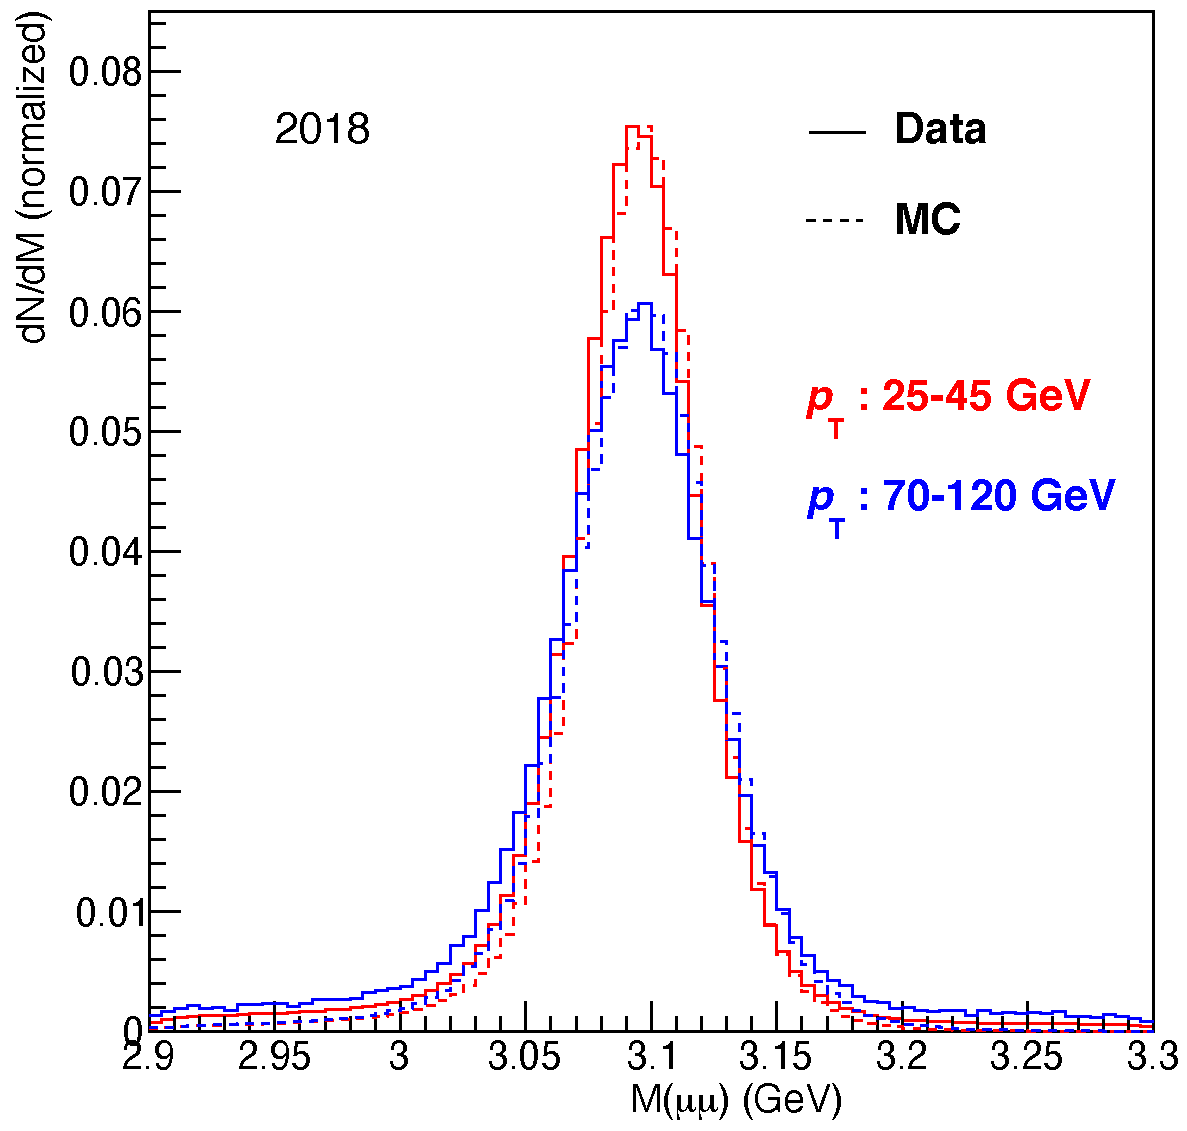
\includegraphics[width=0.485\linewidth]{Figures/chapter2/m_scale2.pdf}
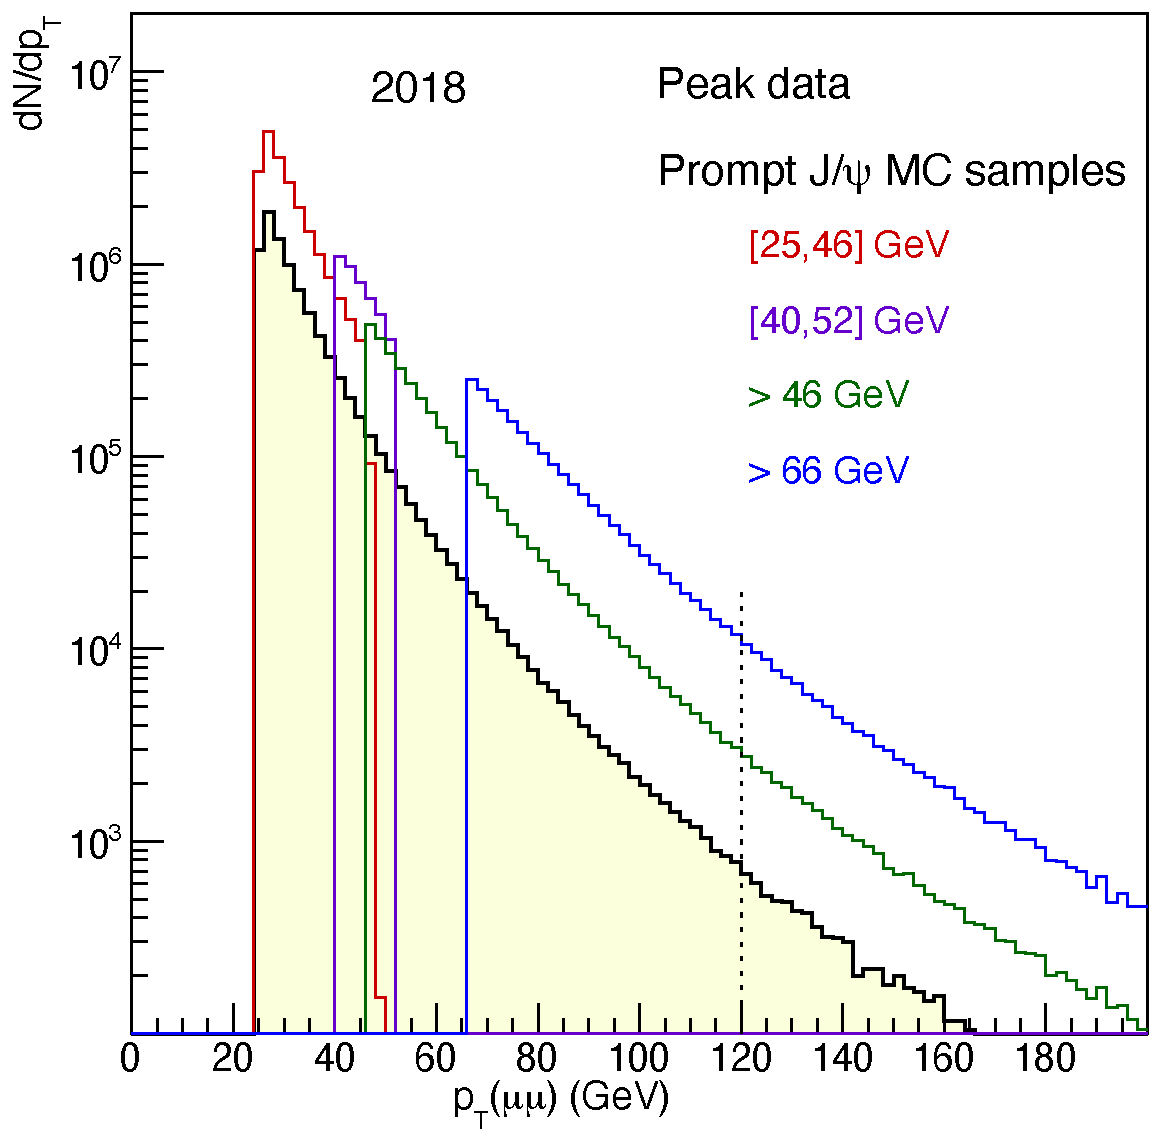
\includegraphics[width=0.475\linewidth]{Figures/chapter2/pt_all2.pdf}
\caption{Left: Invariant mass distribution of the measured (solid histograms) 
and simulated (dashed histograms) prompt dimuons ($|c\tau| < 50\,\mu$m), 
in the 25--45\GeV (red) and 70--120\GeV (blue) \pt ranges.
Right: Measured (black histogram) \pt distribution of the dimuons 
in the prompt \jpsi signal region 
(Peak window: $|c\tau| < 50\,\mu$m and $3.0 < m < 3.2$\GeV), 
compared to the distributions of the four samples of simulated events
(red, purple, green, and blue histograms).}
\label{fig:Jpsi_mass_pt}
\end{figure}

Figure~\ref{fig:Jpsi_mass_pt}-left compares the measured and simulated 
invariant mass distributions of the prompt dimuons ($|c\tau| < 50\,\mu$m)
in the 25--45\GeV (red) and 70--120\GeV (blue) \pt ranges.
There are no continuum background dimuons in the MC samples, 
which are pure (prompt) signal. 
We see that the mass resolution degrades from low to high \pt.
Figure~\ref{fig:Jpsi_mass_pt}-right shows the \pt distributions 
of the measured Peak data (black)
and of the samples simulated in four \pt ranges:
25--46\GeV (``low \pt range", in red),
40--52\GeV (``mid \pt range", in purple),
$>46$\GeV (``high \pt range", in green), and
$>66$\GeV (``highest \pt range", in blue).
It should be kept in mind that the ``data" sample includes contaminations from
\jpsi dimuons produced in B meson decays (even if with $|c\tau| < 50\,\mu$m)
and from ``continuum mass dimuons",
while the simulated samples are pure prompt \jpsi signal.
We have verified that the dimuon kinematic distributions obtained in the
different MC samples are compatible with each other in their common \pt ranges.

\vfill\newpage

Figure~\ref{fig:Jpsi_y} compares the data and MC rapidity distributions,
in the four \pt ranges. The right panel provides an easier comparison of the shapes,
by scaling the MC distributions. The data-MC agreement is quite remarkable.

\begin{figure}[t!]
\centering
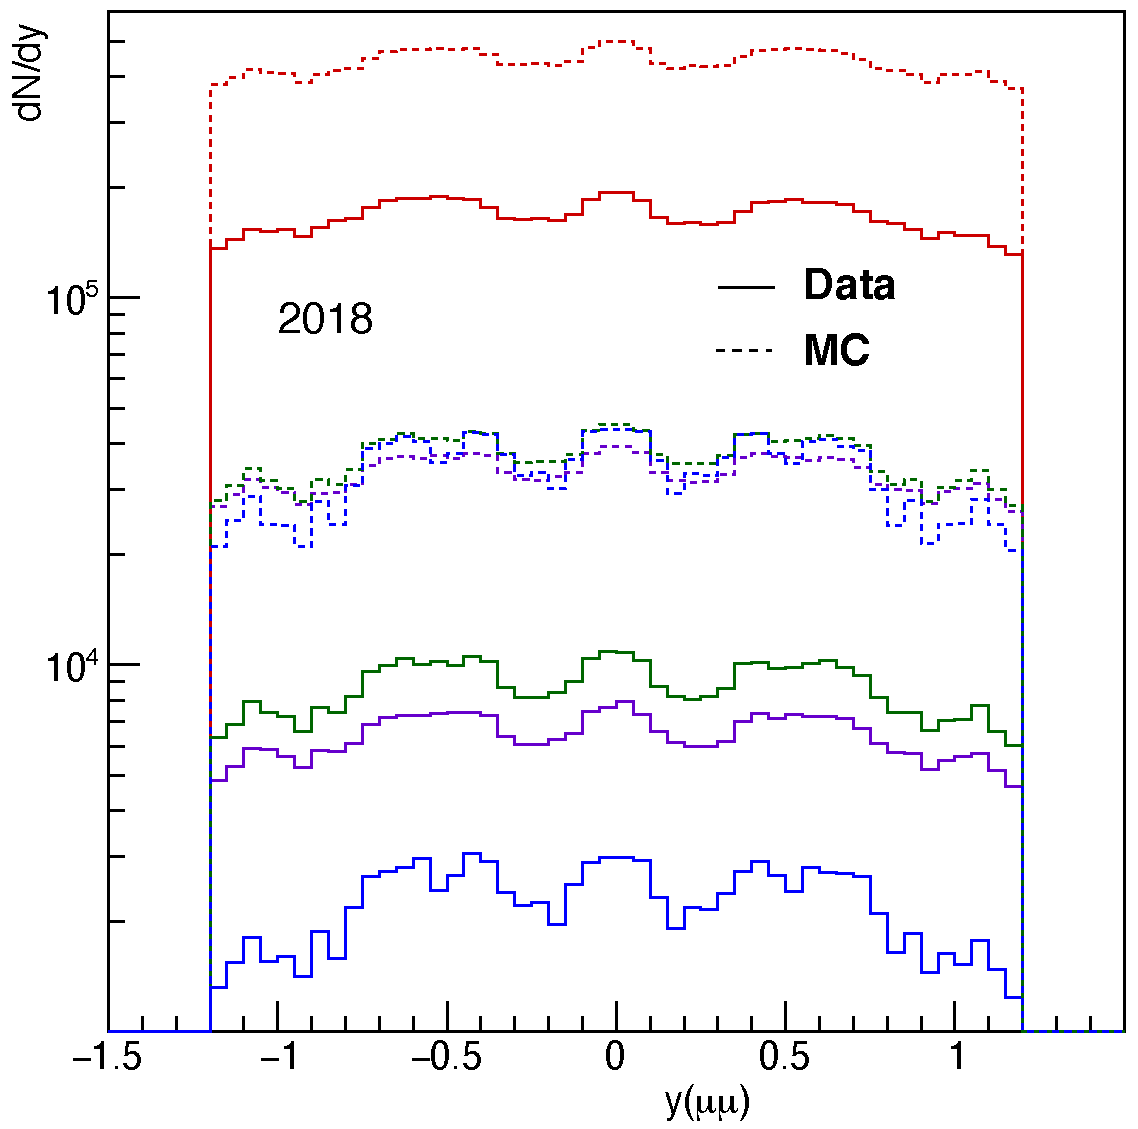
\includegraphics[width=0.47\linewidth]{Figures/chapter2/y_all2.pdf}
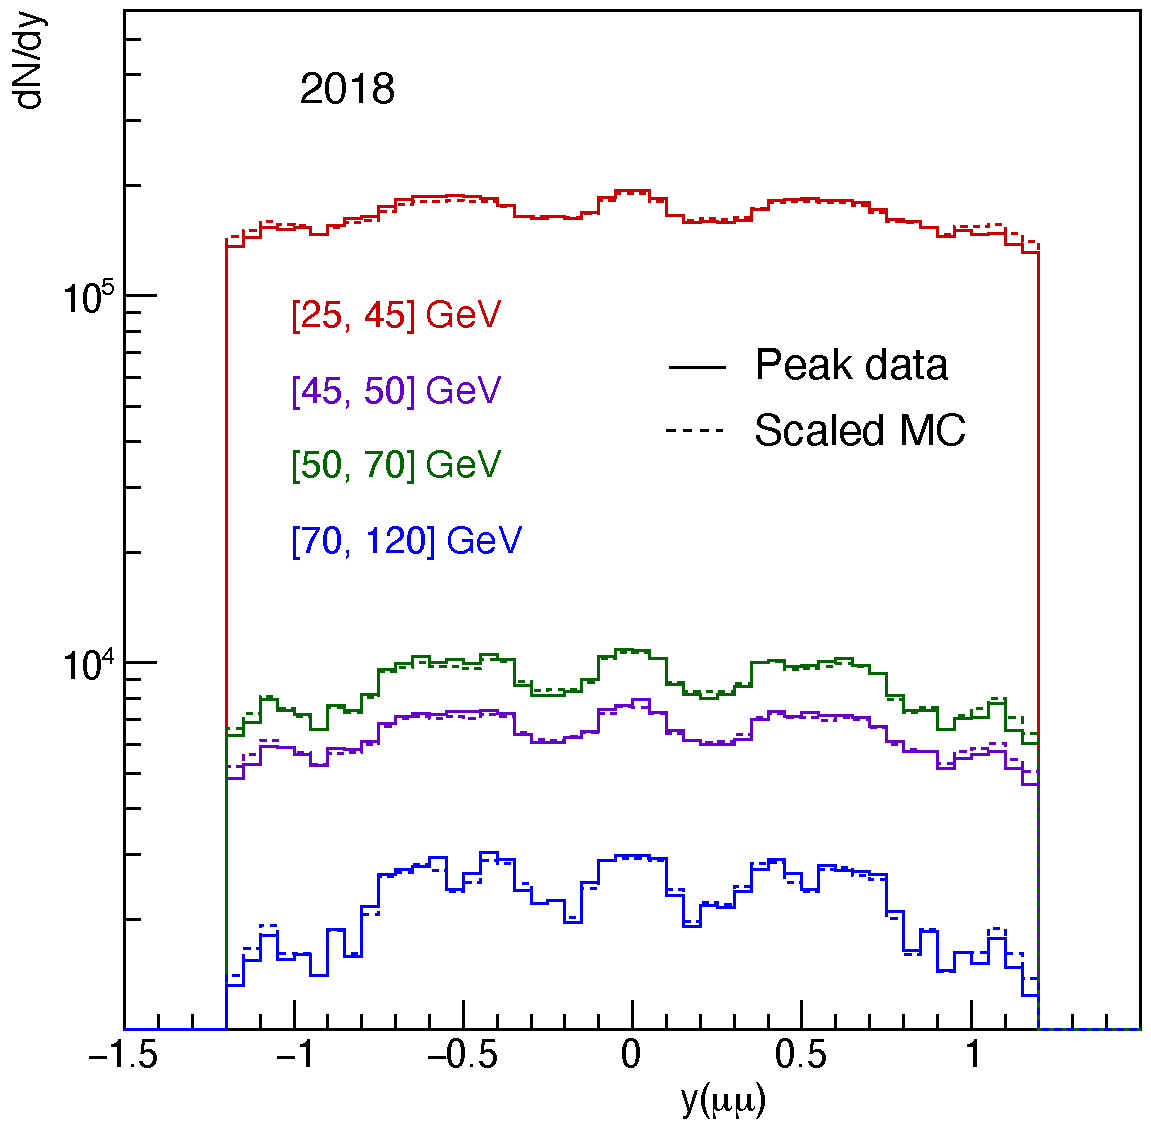
\includegraphics[width=0.47\linewidth]{Figures/chapter2/y_scale2.pdf}
\caption{Rapidity distributions of the measured (solid histograms) 
and simulated (dashed histograms) prompt dimuons in the \jpsi mass region (Peak), 
in four \pt ranges (red, purple, green, and blue histograms), 
before (left) and after (right) rescaling the MC distributions 
for an easier comparison with the data shapes.}
\label{fig:Jpsi_y}
%\end{figure}
\vglue4mm
%\begin{figure}[h]
\centering
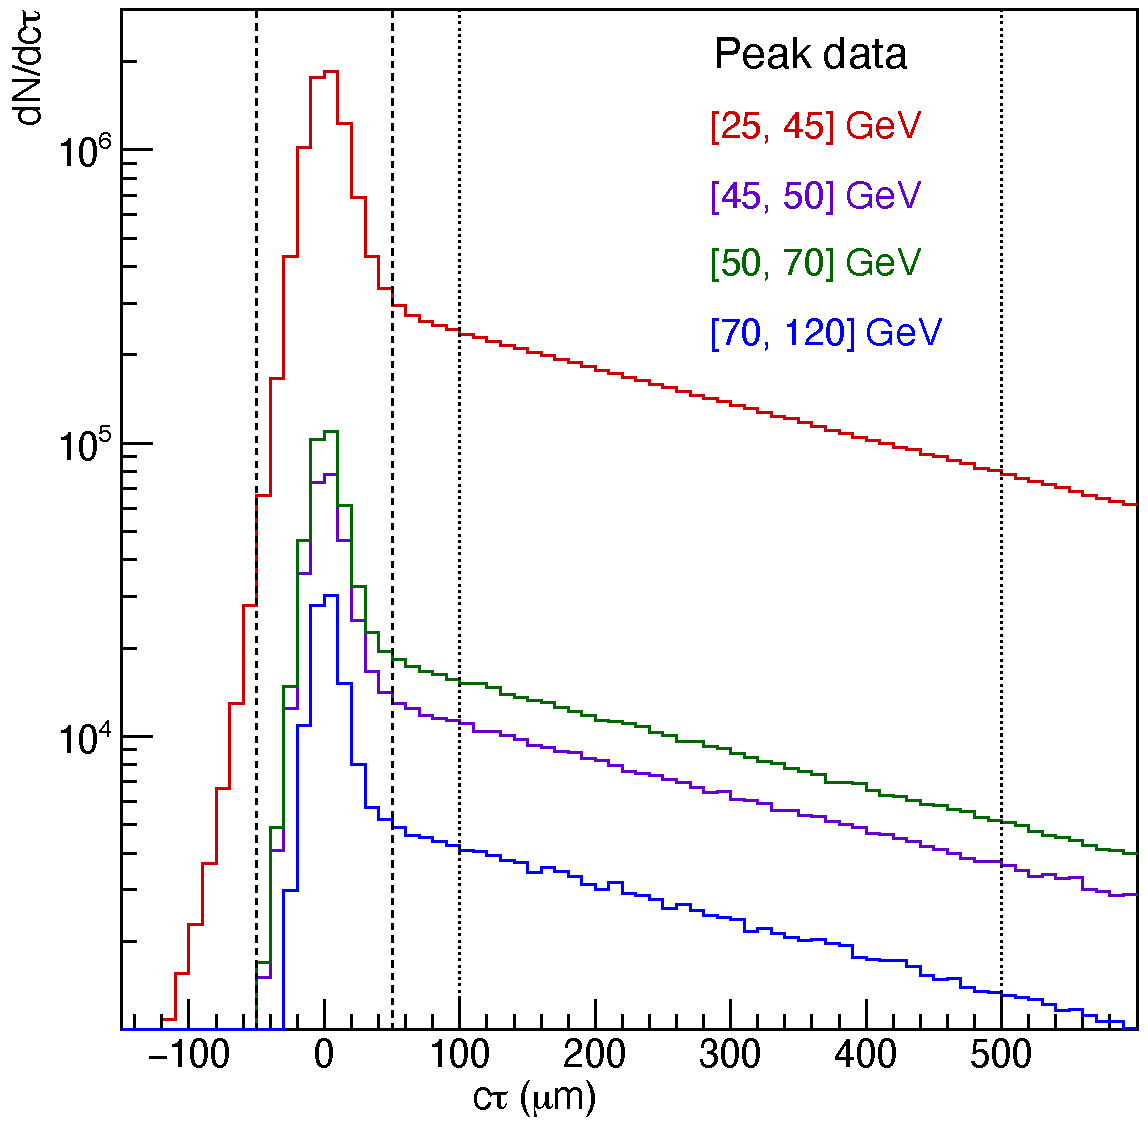
\includegraphics[width=0.47\linewidth]{Figures/chapter2/lt_all2.pdf}
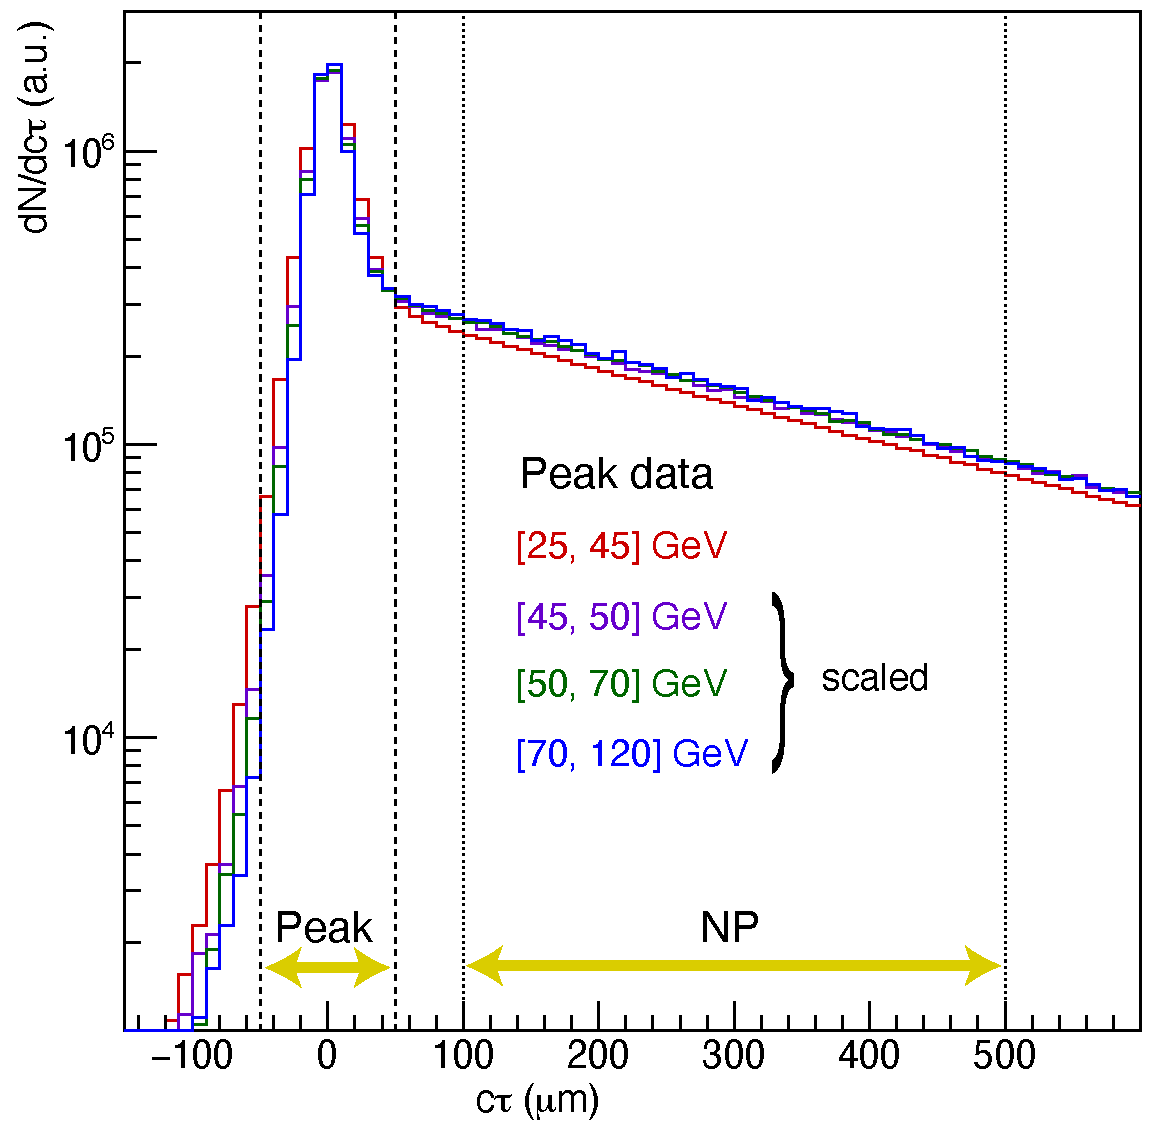
\includegraphics[width=0.47\linewidth]{Figures/chapter2/lt_scale2.pdf}
\caption{Pseudo-proper lifetime distributions of the measured dimuons,
with mass in the 3.0--3.2\GeV window. 
The vertical lines indicate the ``prompt" (dashed) and ``non-prompt" (dotted) windows.}
\label{fig:Jpsi_lifetime}
\end{figure}

As previously mentioned and graphically shown in Fig.~\ref{fig:2D_ctau_vs_mass_map},
the Peak, PR LSB, and PR RSB event samples only include dimuons of 
pseudo-proper lifetime between $-50$ and $+50\,\mu$m.
Instead, the NP event sample is composed of dimuons with 
pseudo-proper lifetime between 100 and 500\,$\mu$m
(and only in the mass window $3 < m < 3.2$\GeV).
Figure~\ref{fig:Jpsi_lifetime} shows the lifetime distribution of
the measured \jpsi dimuons, indicating the prompt and non-prompt windows
with the vertical dashed lines and the two horizontal arrows.
No simulated distributions are shown here because the MC 
is exclusively composed of prompt signal \jpsi events.
We can see that the resolution of the lifetime measurement improves from low to high \pt 
and that the NP fraction increases with \pt and then flattens out.

The next figures provide equivalent illustrations for the \psip case.

\begin{figure}[h!]
\centering
\includegraphics[width=0.485\linewidth]{Figures/chapter2/m_scale_psip.pdf}
\includegraphics[width=0.475\linewidth]{Figures/chapter2/pt_all_psip.pdf}
\caption{Left: Invariant mass distribution of the measured (solid histogram) 
and simulated (dashed histogram) prompt dimuons ($|c\tau| < 50\,\mu$m), 
integrated over \pt.
Right: Measured (black) and simulated (red) \pt distributions of the dimuons 
in the prompt \psip signal region 
($|c\tau| < 50\,\mu$m and $3.57 < m < 3.81$\GeV).}
\label{fig:psip_mass_pt}
%\end{figure}
\vglue4mm
%\begin{figure}[ht]
\centering
\includegraphics[width=0.45\linewidth]{Figures/chapter2/y_all_psip.pdf}
\includegraphics[width=0.45\linewidth]{Figures/chapter2/y_scale_psip.pdf}
\caption{Rapidity distributions of the measured (solid) 
and simulated (dashed) prompt dimuons in the \psip mass region, 
integrated over \pt,
before (left) and after (right) rescaling the MC distributions 
for an easier comparison with the data shapes.}
\label{fig:psip_y}
\end{figure}




